% Cap�tulo 2
\chapter{Fundamentação teórica}

Neste capítulo, são apresentados conceitos teóricos, os quais, embasam todo este trabalho, assim como, servem de fundamentação para análise dos dados obtidos. 

Primeiramente, uma abordagem sobre os aspectos gerais do assunto Processamento de Linguagem Natural  é realizado.

Posteriormente, são apresentadas algumas de suas técnicas, com maior ênfase na análise de sentimento de texto, a qual, tem uma maior relevância para o desenvolvimento deste projeto. 

Em seguida, é demonstrado, sem pormenorizar, o intuito da implementação do serviço web, desenvolvido para propiciar acessibilidade às análises textuais executadas neste trabalho. Além de justificar o motivo da utilização de um framework da linguagem de programação Python, para criação de tal serviço. 

Por fim, são expostas e explicadas as bibliotecas para análise de dados da Python, as quais, servem como dependência para o código fonte do serviço web implementado.

\abrv[PLN -- Processamento de Linguagem Natural]
\section{Processamento de Linguagem Natural}

O principal objetivo do PLN (Processamento de Linguagem Natural) é criar técnicas computacionais com o propósito de entendimento, aprendizado e reprodução de conteúdo linguístico humano. Basicamente, fazer com que computadores compreendam e até interajam com seres humanos, através da linguagem. De acordo com \cite{surveyPLN} esse objetivo, deve ser entendido, como algo não restrito apenas aos desafios da área de IHC (Interação Humano-Computador)\cite{ihc}.

O escopo do PLN engloba áreas de estudo como, linguagens, estatística, psicologia e computação e está contido no domínio da IA (inteligência artificial) a qual, apesar de possuir uma vasta gama de conceitos atribuídos, pode ser definida com o fim de realizar funções que, quando feitas por pessoas, são consideradas inteligentes.

Este termo, inteligência artificial, foi usado inicialmente por John McCarthy em 1956. O tema foi primordialmente estudado em 1945 por Vannevar Bush, apresentado em seu seminário intitulado, \textit{As We May Think} e tem um problema proposto, pelo matemático inglês Alan Turing, em 1950 conhecido como “Teste de Turing”, \cite{IA:06}. 

\subsection{Aplicações e avanços do PLN}

De acordo com \cite{Hirschberg261}, nas últimas duas décadas, a computação linguística vem apresentando um grande crescimento, seja para a área de pesquisa ou para sua aplicação na prática em tecnologias, as quais, são utilizadas em produtos de consumo público. Para citar tais tecnologias, pode-se tomar como exemplo, o Siri (aplicativo assistente pessoal do sistema operacional IOS desenvolvido pela empresa Apple), Cortana (outro aplicativo de assistência pessoal digital criado pela corporação Microsoft) e o Google tradutor (serviço gratuito de tradução instantânea da Google).

Ainda segundo Hirschberg e Manning, no início das pesquisas feitas sobre a computação na linguística, cientistas realizavam seus experimentos, com base apenas, na implementação nos computadores de vocabulários e regras gramaticais das linguagens humanas. O que não se mostrou eficiente, pois não eram levados em consideração aspectos como, a contextualização do que estava sendo analisado, a ambiguidade que as palavras podem apresentar de acordo com as outras que as acompanham num texto, ou seja, ignorava-se a complexidade que uma língua contém.

Porém, esses autores citam quatro fatores que influenciaram o avanço do PLN: aumento da capacidade computacional, a disponibilidade de grandes volumes de dados linguísticos, o desenvolvimento de  \textit{Machine Learning} (aprendizado de máquinas, ou seja, a capacidade computacional de cognição) e um progresso acerca do entendimento da linguagem humana.

O desenvolvimento do PLN pode ser observado nas aplicações a seguir, citadas no trabalho de \cite{Hirschberg261}.

\subsubsection{Tradução automática (\textit{Machine Translation})}

A função de um tradutor é “\textit{... transformar em um idioma o significado expresso por uma passagem de texto em outro idioma.}”, \cite[tradução do autor]{Brown:90}. 
Segundo Brown, a tradução automática feita por computadores, é tão antiga quanto os computadores digitais modernos. No início de seu desenvolvimento os sistemas de regras gramaticais, feitos a mão, não apresentaram resultados satisfatórios. Porém essa tecnologia ganhou relevância quando, pesquisadores da IBM, em 1990, adquiriram e fizeram estudos sobre uma grande quantidade de sentenças nas línguas Inglesa e Francesa. 

Essencialmente, esse estudo permitiu-lhes, coletar dados estatísticos, a respeito de tradução de palavras, e construírem um modelo probabilístico de aprendizado de máquina \cite{Hirschberg261}.

\subsubsection{Sistemas de diálogo falado e Agentes inteligentes conversacionais}

De acordo com \cite{agenteConversacional:17} um agente conversacional, também conhecido como \textit{Chatbot}, é um programa computacional, o qual, tenta processar e criar respostas baseadas na linguagem humana, durante um diálogo.

Os primeiros trabalhos realizados sobre \textit{Chatbots}, usaram apenas técnicas simples de correspondência entre diálogos em formato textual. Por exemplo, se um emissor, de um lado, responde “sim”, a uma determinada pergunta feita pelo outro emissor, uma ação pré estabelecida no \textit{Chatbot} é processada e executada, portanto, não levava em consideração o contexto em que aquele diálogo estava inserido. Isso acontecia, pelo fato do sistema ser fechado, ou seja, apenas palavras e expressões prescritas nele eram interpretadas, o restante era ignorado.

Com o passar do tempo, a tecnologia criada para os agentes conversacionais evoluiu de diálogos textuais para diálogos falados. Atualmente é possível perceber seu progresso, ao observar aplicações criadas para dispositivos móveis e outras plataformas. 

Tais aplicativos executam tarefas de assistência pessoal, como, Siri e Cortana, e também são integrados em sistemas robóticos de interação entre humanos e robôs \cite{roboticaAssistida:15}, os quais, apresentam um intuito educativo, assim como, reabilitação de pessoas com deficiência e cuidados médicos.

\subsubsection{Leitura automática e sumarização de informação (\textit{Machine reading})}

A quantidade de literaturas científicas está crescendo exponencialmente, como exemplifica \cite{Hirschberg261}, a biblioteca nacional de medicina dos Estados Unidos \textit{U.S. National Library of Medicine} apresenta um crescimento exponencial no número de obras publicadas.

Em uma palestra, filmada e divulgada na internet \cite{drauzioYoutube}, realizada em decorrência de um parceria do site do Dr. Drauzio Varella com a \textit{International Business Machines} (IBM), intitulada como “Computação cognitiva no reconhecimento de exames de Imagens”, o tema é abordado, citando como exemplo um especialista qualquer de alguma área médica.

Nesse exemplo, é dito que é humanamente impossível este especialista se manter atualizado, de acordo com o grande volume de publicações que são feitas atualmente, em um tempo hábil. E que para resolver tal problema, a IBM desenvolveu a Watson. Uma plataforma de serviços cognitivos para negócios, disponíveis na internet.

A função da Watson, na situação em discussão, é ler e processar uma enorme quantidade de informações, desde trabalhos científicos sobre a especialidade do médico, até históricos de seus pacientes e devolver ao especialista dados sumarizados e estruturados, além de novos conhecimentos para auxílio da sua tomada de decisão, em um curto espaço de tempo.

Portanto, o que caracteriza o \textit{Machine reading} é a idéia de que máquinas possam adquirir inteligência suficiente, para integrar e sumarizar a enorme quantidade de textos disponíveis, lendo-lhes.

\subsubsection{Mineração de dados em redes sociais}

Atualmente nesta era da informação, onde uma imensa quantidade de dados é gerada constantemente, o desenvolvimento das redes sociais alavancou ainda mais a variedade e o volume dessas informações.

As redes sociais, inclusive, revolucionaram a forma com que empreendedores, jornalistas, políticos, anunciantes e médicos obtém dados acerca de seus produtos de trabalho, além de como utilizam essas informações, na prática, para auxílio em tomadas de decisões nos seus negócios.

Como dito por \cite{Hirschberg261} a coleta de dados sobre produtos e serviços pode ser analisada com a intenção de prever seus preços e auxiliar as campanhas de anúncio desenvolvidas em cima desses produtos. Comunidades e fóruns políticos geram informações que podem ser exploradas para que levantamentos sobre uma determinada campanha política sejam feitos.

Existem desvantagens na mineração de dados em redes sociais. Como é o caso de problemas com as informações particulares dos usuários. Nessa situação, interesses entre partes entram em conflito, já que, os usuários tendem a exigir sua privacidade com a proteção de parte ou todo o seu conteúdo e pesquisadores e empresas tendem a querer ter acesso a isso. O que leva as redes sociais, tal como o Twitter, a bloquearem esses dados para acesso dos pesquisadores interessados, além de diminuírem a porção e a velocidade de aquisição, mesmo das informações que estão disponíveis.

Outro desafio em \textit{Mining social media} é o de discernimento entre informação  falsa e verdadeira, visto que, não existe uma forma completamente eficaz de validar e comprovar como verdade ou mentira, o que um usuário posta a respeito de si ou se avaliações feitas em páginas de empresas correspondem a realidade da opinião pública, por exemplo.

Embora haja problemas no objeto de estudo em questão, redes sociais como Twitter, Facebook, YouTube e fóruns de discussão possibilitam acesso de dados para análise de informações demográficas, sobre interações sociais, sobre possíveis epidemias e a opinião do público em geral acerca de um tema ou acontecimento.

\subsection{Técnicas do PLN}

Segundo \cite{tecnicasPLNRanjan:16} , ao longo dos anos, foram desenvolvidas várias aplicações que utilizam o Processamento Natural de Linguagem. Exemplos são, reconhecimento de voz, tradução automática, busca de informações, sumarização de textos, entre outras.

Para desenvolvimento de tais aplicações, há a necessidade de emprego de técnicas, as quais, permitem com que esses problemas relacionados ao PLN sejam resolvidos. O propósito da execução delas é o de: 

\begin{itemize}
\item transformar dados não estruturados, de linguagem natural, em dados estruturados, para que os algoritmos de PLN consigam recebê-los como entrada e processá-los, gerando uma saída satisfatória para as aplicações relacionadas;

\item garantir a essas informações estruturadas, a existência de atributos que apresentem relação com o objeto de estudo em questão;

\item  imputar esses dados em algoritmos de PLN.

\end{itemize}

As fases do processo de execução do PLN, ou seja, a “canal” por onde as sentenças em linguagem natural são imputadas, consiste de várias técnicas, porém a seguir duas são apresentadas: Análise gramatical e \textit{Parsing}.

\subsubsection{Análise morfológica}

Na língua inglesa, a sentença \textit{Part of Speech}, com acrônimo POS, significa literalmente, em língua portuguesa, “Parte do Discurso”. Mas se refere ao conceito de análise morfológica, do português.

Enquanto que a palavra \textit{Tagging} corresponde ao verbo marcar, em inglês, no tempo verbal \textit{Present Continuous}. Tempo esse, que indica uma ação que está acontecendo no presente ou irá acontecer no futuro. Então ao unir estas informações tem-se que, análise morfológica reflete que uma análise morfológica será ou está sendo feita e que o resultado dessa análise será marcado, anexado a algum lugar.

Para \cite{tecnicasPLNRanjan:16} a análise morfológica é a fase de trabalho que antecede a do \textit{Parser}. Tal fase é executada com o objetivo de classificar palavras de sentenças, em uma das classes de palavras existentes, e “rotular” estas, palavras de sentenças, com sua classificação morfológica.

Para exemplificar, este processo consiste em, obter uma determinada sentença; segmentar suas palavras; e classificá-las, atribuindo rótulo a elas, definindo se uma palavra é um verbo, um artigo, uma preposicão, etc.

Embora na análise morfológica a análise morfológica de um texto, seja realizada em palavras individualmente, elas são dependentes e precisam estar em contexto entre si, para que haja uma análise correta. Pois o significado e a classe de palavras, a qual pertence uma palavra, muda de acordo com as outras que estão ao seu redor na sentença. Como demonstra as seguintes frases: 

\begin{itemize}

\item  - “Esse cão não para de latir!”
\item  - “O latir daquele cão é alto.”

\end{itemize}

A palavra “latir” da primeira frase, pertence a classe dos verbos, porém a mesma palavra na segunda frase é substantivada pela precessão do artigo, definido e masculino, “O”.

\subsubsection{\textit{Parsing}}

O conceito de \textit{Parsing} é aplicado em outros domínios da ciência da computação, além do PLN, como na construção de compiladores capazes de transformar código fonte em código executável por uma máquina. Nesta seção é apresentado o conceito de  \textit{Parsing} dentro do domínio do PLN.

Segundo \cite{tecnicasPLNRanjan:16} a etapa básica do processamento de linguagem natural é atingida quando uma \textit{parse tree}, ou árvore de análise, é gerada. Um parser recebe como entrada sentenças ou sequências de tokens em linguagem natural, divide-as em partes menores, o que permite uma melhor identificação da sintaxe de cada elemento presente na entrada. Assim, com ajuda de regras gramaticais definidas, é gerado como saída do parser, uma árvore de análise (\textit{parse tree}).

\section{Análise de sentimento}

Análise de sentimento é uma subárea do processamento natural de linguagem, também conhecida como mineração de opinião. A idéia principal desse tipo de análise é a de desenvolver ferramentas capazes de extrair informações subjetivas de textos em linguagem natural como opiniões e sentimentos. Assim, geram-se informações estruturadas, automaticamente, que podem ser usadas em processos de tomada de decisão ou de obtenção de conhecimento, acerca de algum objeto de interesse. \textit{“O objetivo da análise de sentimento é, portanto, definir ferramentas automáticas capazes de extrair informações subjetivas para criar conhecimento estruturado.”} \cite[tradução do autor]{Pozzi20171}.

Assim como o PLN a análise de sentimento também é aplicada em diversas áreas da sociedade. Negócios são beneficiados com a utilização de aplicações que fazem análise de sentimentos, pois toda empresa deseja satisfazer os desejos de seus consumidores, seja otimizando seus serviços ou inovando-se. Previsões acerca de algum assunto podem ser feitas, como estimar como o mercado de ações irá se comportar ou quem irá ganhar a próxima eleição política. Como também, ser aplicada na medicina para conseguir conhecimento sobre questões da saúde humana \cite{twitterDiabetes2017}.

Existem duas abordagens principais de análise de sentimento: a abordagem baseada em léxico e a abordagem que utiliza aprendizado de máquina, do inglês \textit{Machine Learning}. A figura \ref{fig:arvoreAnaliseSentimental} mostra um diagrama em árvore, apontando as áreas que contêm a análise de sentimento.

\begin{figure}[h]
    \centering
    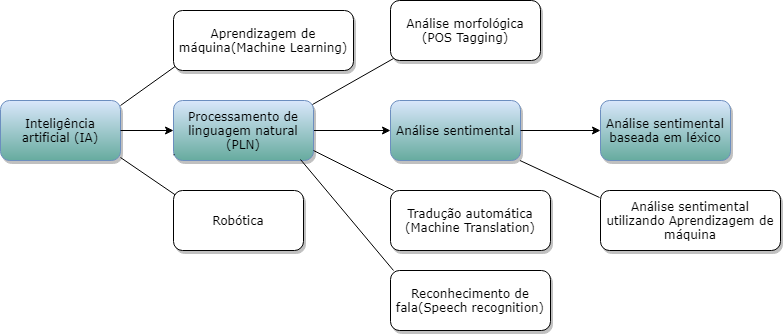
\includegraphics[width=0.95\textwidth]{imagens/arvoreAnaliseSentimental.png}
    \caption {Diagrama em árvore mostrando as áreas que estão relacionadas à análise de sentimento.}
    \source{Fonte: Criado pelo autor com a ferramenta draw.io (2018)}
    \label{fig:arvoreAnaliseSentimental}
\end{figure}

A análise de sentimento baseada em léxico, recebe como entrada um determinado conteúdo em linguagem natural, seja ele composto de palavras, frases ou sentenças completas. Em seguida divide-se essa entrada em partes menores chamadas de \textit{tokens} em um processo chamado \textit{tokenization}. Após isso, são somadas a quantidade de vezes com que elementos dessa entrada se repetem, um modelo conhecido como \textit{Bag of words} \cite{bagOfWords}. Por fim, um banco de dados com palavras que contêm valores de sentimentos pré estabelecidos é consultado e então é computado o valor sentimental daquele texto de entrada. Por exemplo se o resultado final for igual a um número negativo, o texto tem sentimento negativo, se o resultado der igual a zero, sentimento neutro e resultado com valor positivo, o sentimento é tido como positivo. O processo de análise é esquematizado na figura \ref{fig:fluxoAnaliseLexical}. 

\begin{figure}[h]
    \centering
    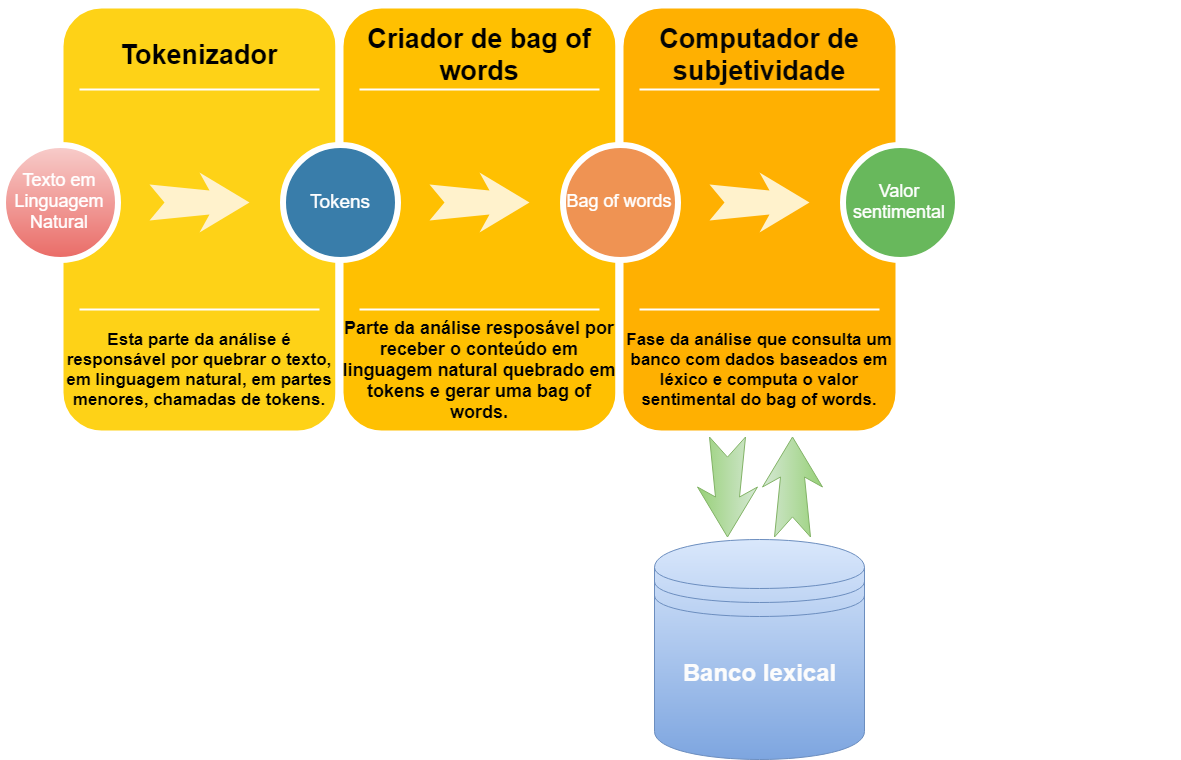
\includegraphics[width=13cm, height=8cm]{imagens/Figura-de-fluxo-analise-lexical.png}
    \caption {Fluxo de análise de sentimento baseada em léxico.}
    \source{Fonte: Criado pelo autor com a ferramenta draw.io (2018)}
    \label{fig:fluxoAnaliseLexical}
\end{figure}

Na abordagem baseada em aprendizado máquina, ao obter, por exemplo, mensagens do Twitter classificadas como negativas ou positivas, é possível criar e “treinar” um algoritmo classificador para que dada uma próxima mensagem, esse algoritmo possa classificá-la como positiva ou  negativa. Geralmente nessa abordagem são utilizadas redes neurais.

Dessas duas formas de se analisar sentimentalmente algo em linguagem natural, a baseada em léxico apresenta menos complexidade, porém a que utiliza \textit{Machine Learning} gera resultados mais acurados principalmente em textos que contenham figuras de linguagem como o sarcasmo.  

\section{Desenvolvimento de um serviço web}

Com o objetivo de expor o modelo de análise de sentimento que este trabalho se propõe a fazer, é desenvolvido um serviço web com o intuito, também, de pôr em prática toda a pesquisa teórica realizada.

De acordo com \cite{webService:2004} um serviço web estabelece um padrão de comunicação entre programas computacionais, que podem estar rodando em diferentes plataformas ou tecnologias.

Para implementação de tal serviço, o \textit{framework} Flask, da linguagem de programação Python, é utilizado.

\subsection{Flask: \textit{framework} Python para desenvolvimento web}

Flask é um \textit{framework} da linguagem de programação Python, desenvolvido na Pocoo (organização composta por desenvolvedores da comunidade da Python), por um de seus membros, Armin Ronacher no ano de 2010. 

Esse \textit{framework} foi planejado para ser escalável e de fácil utilização. No site da tecnologia, o Flask está definido como sendo um \textit{microframework}. A idéia com essa definição é de que, com o Flask, um desenvolvedor obtenha uma ferramenta com funcionalidades essenciais ao desenvolvimento de aplicações para a web e posteriormente, se necessário, possa adicionar ou criar módulos para essa estrutura.

O Flask tem como dependência duas bibliotecas externas a ele: a Jinja2 e a Werkzeug WSGI toolkit (interface padrão entre serviços web e aplicações escritas em Python, para garantir portabilidade).

\subsubsection{Justificativa}

Embora existam outros \textit{frameworks} Python mais robustos para desenvolvimento web como Django e Pyramid, a escolha deste se deu por conta da simplicidade arquitetural que o serviço web desenvolvido neste trabalho requer.

Além desse motivo os seguintes requisitos contidos no Flask são levados em consideração:
\begin{itemize}

\item servidor web embutido;
\item suporte para testes unitários de aplicação;
\item fácil implementação de uma arquitetura RESTful para uma API;
\item suporte para uso de \textit{cookies} (sessões no lado cliente da aplicação);
\item possui arquitetura modular;
\item acompanha uma documentação cheia de exemplificações, inclusive com aplicações já implementadas e prontas para uso;
\item fácil instalação da aplicação em um servidor;
\item fácil configuração;
\item possui funcionalidades para utilização do protocolo HTTP.

\end{itemize}

\subsection{Bibliotecas Python para análise de dados}

O código do sistema implementado neste trabalho, depende de algumas bibliotecas Python. Entre elas, a seguir são descritas as quatro principais. Duas para lidar com o processamento natural de linguagem (NLTK e pandas), uma para facilitar acesso a API da rede social (python-twitter) e uma para facilitar as transações com o banco de dados MongoDB (PyMongo).

\subsubsection{Natural Language Toolkit — NLTK}

NLTK é uma biblioteca Python, desenvolvida para lidar com atividades relacionadas à dados sobre a linguagem humana. Além de conter bibliotecas para processamento de linguagem natural como classificação de textos, tokenização, redução de palavras a seus radicais (\textit{stemming}), \textit{parsing}, entre outras.

\subsubsection{Python Data Analysis Library — pandas}

pandas é uma biblioteca de código aberto, patrocinada pela organização NUMFOCUS, desenvolvida para garantir alta performance e facilidade de uso para desenvolvedores Python. Seu objetivo é fornecer, a este desenvolvedor, ferramentas que ajudem nas questões que envolvem estrutura de dados e análises de dados, de uma forma que, o foco seja mais nos problemas da pesquisa aos da programação.

\subsubsection{python-twitter}

O Twitter expõe uma API aos desenvolvedores, e esta biblioteca foi desenvolvida com o objetivo de facilitar a conexão e uso dos serviços disponíveis, para programadores Python. Funciona com as versões Python 2.7+ e Python 3.

\subsubsection{PyMongo}

PyMongo é uma ferramenta responsável por trabalhar com banco de dados, sendo a biblioteca oficial para acesso ao MongoDB via código Python. Em PyMongo, a estrutura de dados, Dicionário, é usada para representar os documentos no banco, não somente relacional, MongoDB. 

Esse documentos, podem conter tipos de dados complexos como \textit{datetime}, o que com o auxílio do PyMongo pode ser automaticamente convertido para objetos Python. O que facilita a lógica do desenvolvimento, fazendo mais operações com menos código.



